\documentclass[crop,tikz]{standalone}
\usetikzlibrary{backgrounds}
\colorlet{blue}{cyan}
\tikzset{
  inverted/.style = {
    color=white,
    background rectangle/.style={fill},
    show background rectangle
  }
}
\usepackage{pgfplots}
\pgfplotsset{compat=1.13}

% Field lines and lines of constant potential for an electric dipole.
%
% Inspired by the expressions given in Fließbach, "Arbeitsbuch zur
% Theoretischen Physik", example 11.7.

\pgfplotsset{
  inverted/.style = {
    every axis legend/.append style={
      draw=white,
      fill=black,
      text=white
    }
  },
}

\begin{document}

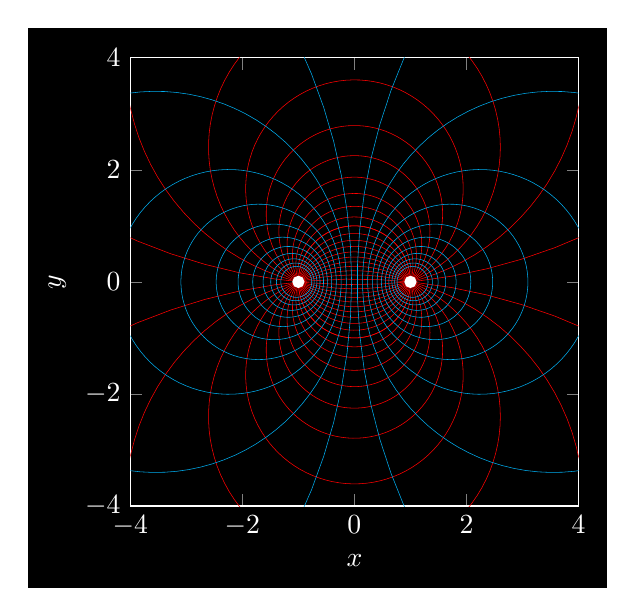
\begin{tikzpicture}[inverted,inverted]
  \pgfmathsetmacro{\numberoffieldlines}{10};
  \pgfmathsetmacro{\numberofpotentiallines}{10};
  \pgfmathsetmacro{\chargepos}{1};
  \pgfmathsetmacro{\sigmamin}{0.1}; % minimum sigma
  \pgfmathsetmacro{\sigmamax}{pi/2}; % maximum sigma
  \pgfmathsetmacro{\taumin}{0.1}; % minimum tau
  \pgfmathsetmacro{\taumax}{2}; % maximum tau
  \pgfmathsetmacro{\remin}{-4*\chargepos};
  \pgfmathsetmacro{\remax}{-\remin};
  \pgfmathsetmacro{\immin}{-4*\chargepos};
  \pgfmathsetmacro{\immax}{-\immin};
  \begin{axis}[inverted,
    axis equal image,
    xmin={\remin}, xmax={\remax},
    ymin={\immin}, ymax={\immax},
    xlabel={$x$},
    ylabel={$y$},
    samples=100,
    domain=0:360,
    declare function = {
      phir(\a,\c) = sqrt(\c^2 - \a^2); % radius
      phix(\x,\c,\a) = phir(\a,\c)*cos(\x) + \c*\a;
      phiy(\x,\c,\a) = phir(\a,\c)*sin(\x);
      coth(\x) = 1 + 2/(exp(2*\x) - 1);
      fc(\n,\nmax) = coth(\taumin + \n/\nmax*(\taumax - \taumin)); % calculates c
      Er(\a,\c) = sqrt(\a^2 + \c^2); % radius
      Ex(\x,\c,\a) = Er(\a,\c)*cos(\x);
      Ey(\x,\c,\a) = Er(\a,\c)*sin(\x) + \c;
      pc(\n,\nmax) = cot(deg(\sigmamin + \n/\nmax*(\sigmamax - \sigmamin))); % calculates c
    },
    ]
    % field lines
    \pgfplotsinvokeforeach{0,...,{\numberoffieldlines}}{
      \addplot[red,very thin] (
        {Ex(x, pc(#1,\numberoffieldlines), \chargepos)},
        {Ey(x, pc(#1,\numberoffieldlines), \chargepos)}
      );
      \addplot[red,very thin] (
        {Ex(x, -pc(#1,\numberoffieldlines), \chargepos)},
        {Ey(x, -pc(#1,\numberoffieldlines), \chargepos)}
      );
    }
    % lines of constant potential
    \pgfplotsinvokeforeach{0,...,{\numberofpotentiallines}}{
      \addplot[blue,very thin] (
        {phix(x, fc(#1,\numberofpotentiallines), \chargepos)},
        {phiy(x, fc(#1,\numberofpotentiallines), \chargepos)}
      );
      \addplot[blue,very thin] (
        {phix(x, -fc(#1,\numberofpotentiallines), \chargepos)},
        {phiy(x, -fc(#1,\numberofpotentiallines), \chargepos)}
      );
    }
    % charges
    \addplot[only marks,mark=*] coordinates {
      ({ \chargepos},0)
      ({-\chargepos},0)
    };
  \end{axis}
\end{tikzpicture}
\end{document}
